\documentclass{article}
\usepackage[utf8]{inputenc}

%additional usepackages
\usepackage{amsmath}
\usepackage{eufrak}
\usepackage{tikz}
\usepackage{ amssymb }
\usepackage{import}
\usepackage[ruled,vlined]{algorithm2e}
\usepackage{booktabs}
\usepackage[capposition=top]{floatrow}
\usepackage{scrextend}
\usepackage{csquotes}
\usepackage{graphicx}


% bibliography
\usepackage{biblatex}
%\addbibresource{soda.bib}


% margins
\usepackage[margin=1.05in]{geometry}

%new commands
\newcommand{\ances}{AN_{A}^{\mathcal{G}}}
\newcommand{\anc}{\mathbf{AN}^{\mathcal{G}}}
\newcommand{\dec}{\mathbf{DE}^{\mathcal{G}}}
\newcommand{\dsep}{\text{ \textit{d}-sep }}
\newcommand{\dseperation}{\text{ \textit{d}-seperation}}
\newcommand{\nodes}{\mathbf{V}}
\newcommand{\parents}{\mathbf{PA}^{\mathcal{G}}}
\newcommand{\parentsNew}{\mathbf{PA}^{\mathcal{G^{*}}}}
\newcommand{\summ}{\frac{1}{n}\sum_{i=1}^{n}}


\newcommand{\children}{\mathbf{CH}^{\mathcal{G}}}

\newcommand{\graph}{\mathfrak{C}}
\newcommand{\E}{\mathbb{E}}
\newcommand{\std}{\mathbf{std}}
\newcommand{\R}{\mathbb{R}}
\newcommand{\G}{\mathcal{G}}
\newcommand{\lra}{\Leftrightarrow}

\newcommand{\la}{\leftarrow}
\newcommand{\ra}{\rightarrow}

\newcommand{\rp}{\right)}
\newcommand{\lp}{\left(}

%%%% INDEPDENT SIGN %%%%

\makeatletter
% Taken from http://ctan.org/pkg/centernot
\newcommand*{\centernot}{%
  \mathpalette\@centernot
}
\def\@centernot#1#2{%
  \mathrel{%
    \rlap{%
      \settowidth\dimen@{$\m@th#1{#2}$}%
      \kern.5\dimen@
      \settowidth\dimen@{$\m@th#1=$}%
      \kern-.5\dimen@
      $\m@th#1\not$%
    }%
    {#2}%
  }%
}
\makeatother

\newcommand{\independent}{\perp\mkern-9.5mu\perp}
\newcommand{\notindependent}{\centernot{\independent}}

%%%%% INDEPENDENT SIGN END %%%%%

\newcommand{\X}{\mathbf{X}}
\newcommand{\Ls}{\mathbf{L}}
\newcommand{\D}{\mathbf{D}}
\newcommand{\W}{\mathbf{W}}

\newcommand{\x}{\mathbf{x}}
\newcommand{\ls}{\mathbf{l}}
\newcommand{\ds}{\mathbf{d}}
\newcommand{\w}{\mathbf{w}}

\newcommand{\rr}{\mathbf{r}}
\newcommand{\RR}{\mathbf{R}}

\newcommand{\ones}{\mathbf{1}}

\DeclareMathOperator*{\argmax}{arg\,max}
\DeclareMathOperator*{\argmin}{arg\,min}


\setlength{\parindent}{0em}
\setlength{\parskip}{0.25cm}

\title{Stock Picking In an Environment of Structural Breaks}
\author{Jeppe Søndergaard Johansen (pcv439)}
\date{August 2019}

\makeindex

\begin{document}

\maketitle

\section{Abstract}

NOTER:
- JEG MANGLER INTRODUKTION

- JEG MANGLER LITTERATUR REVIEW (SKAL VÆRE KORT) (GIV GERNE FORSLAG TIL GODE PAPIRER)

- JEG SKAL OGSÅ LIGE FINPUDSE KONKLUSIONEN

This paper investigates stock picking in an environment of structural breaks. A structural break, in this paper, is defined as an event that upends the data generating process of stock returns. I stride to find an algorithm that performs well at choosing the single stock with highest sharp ratio in each period.

I use data of 11 stocks for the past 30 years. First the data is presented, using graphs and summary statistics, for the individual stocks.

Next I present a structural causal model that attempts to model stock returns under a regime of structural breaks. I identify the parameters necessary for sampling from the structural model. Using the real data collected, I use log-likelihood estimation to find the parameter values. I simulate a data set of $11$ stocks with $2.000.000$ rows containing slightly less than $10.000$ structural breaks.

I move onto present three different algorithms for predicting the Sharpe ratio in a given time period. These being a deep learning model called LSTM, and two simpler algorithm using rolling estimations of Sharpe ratios. I discuss the different properties, and how each model should be trained and tuned.

Using the simulated data set i compare the three different algorithms and their capacity to accurately predict the Sharpe ratio of individual stocks. Using the best model i investigate the performance on the real data set comparing to different benchmarks. Using not only summary statistics of the different strategies for stock picking, but I also plot the counter factual investment strategies, and make a Monte Carlo simulation for comparing the performance of the different strategies. I find the best performing model to be the one using a rolling Sharpe ratio. Comparing to a tangency portfolio the Sharpe ratio is about twice as high: $0.12563$ compared to $0.05545$

In the end i discuss the challenges of tuning, training and selecting algorithms, and what this might entail for using in-sample-machine learning for developing trading algorithms. In more depth i discuss the challenges of using LSTM algorithms, and the limitations of my computer setup for efficiently training such an algorithm. Finally I discuss the value of creating controlled environments for trading algorithm development.

\tableofcontents

\pagebreak

%\input{chapters/introduction.tex}

\section{Data}


\section{The model}\label{sec:model}

Before investigating the model in more depth some elaboration of the notation used in this paper: $\Omega$ is used to denote covariance matrices, with individual elements of $\Omega$ denoted $\sigma^{2}_{i,j}$, and noting that the variances are the diagonal of the matrix, these being denoted = $\sigma^{2}_{i,i} = \sigma^{2}_{i}$. Moving on,  $\mu = (\mu_1, \mu_2, \cdots \mu_{k})$ is used for denoting a vector of $k$ expected returns. It should be noted that $\Omega$ is a $k\times k$ matrix, or rather the length $\mu$ should correspond to the size of the symmetric covariance matrix. The returns at time $t$ are denoted as $\rr^{(t)} = (r_1^{(t)}, r_2^{(t)}, \cdots, r_k^{(t)})$. In general the stochastic variables will be upper case, and the realization will be denoted in lower case. such that $\RR^{(t)}$ is a stochastic vector, and $\rr^{(t)}$ is vector of realized returns. Let $\bar{r}$ denote the risk free asset, and let $\ones$ denote a vector of 1's of length $k$). Sharpe ratio is denoted $sr$. Vectors will be denoted in bold when possible.

\subsection{CAPM}

As alluded to in the introduction, in CAPM it's assumed that the returns of stocks are drawn $i.i.d$ from an multivariate distribution with fixed mean $\mu$ and covariance matrix $\Omega$. Assuming that the returns are normally distributed the structural model driving the data generating process can be summed up into a single equation:

\begin{equation}
    \RR^{(t)} \sim N(\mu, \Omega)
\end{equation}

\subsection{Model formulation with structural breaks}

As alluded to in chapter \ref{sec:data}, the assumption, that a single covariance matrix and expected returns can represent the data generating process seems very unlikely. There are in general two approaches to this problem:

\begin{enumerate}
    \item Assuming the covariance matrix and expected returns steadily moves over time, something akin to a AR process.
    \item Assuming in each period with a certain probability a structural break will occur, and this will generate a vector of expected returns vector and a covariance matrix.
\end{enumerate}

In this paper the ladder option is investigated. This leads to the following structural model:

First a variable $b^{(t)}\in \{0,1\}$ is drawn which represent a structural break. If $b=1$ a structural break is assumed. The parameter $p$ in equation \ref{eq:structuralbreak} denotes the probability of a structural break.

\begin{equation}\label{eq:structuralbreak}
    b^{(t)} = bern(p)
\end{equation}

If $b = 1$ a new covariance matrix, and expected returns vector is drawn, where $d_{\mu}, d_{\Omega}$ are the distributions of the vector of expected returns  and covariance matrix. These distributions will be addressed later.

\begin{equation}
    \mu^{(t)} \sim d_{\mu} \qquad \Omega^{(t)} \sim d_{\Omega}
\end{equation}

If $b=0$ the covariance matrix and expected returns vector is equal to the previous:

\begin{equation}
    \mu^{(t)} = \mu^{(t-1)} \qquad \Omega^{(t)} = \Omega^{(t-1)}
\end{equation}

Lastly we draw the returns just as in the regular CAPM formulation, with the caveat $\mu$ and $\Omega$ contains a top-script $t$:

\begin{equation}
    \RR^{(t)} \sim N(\mu^{(t)}, \Omega^{(t)})
\end{equation}

So in any given period the tangency portfolio can be calculated, however this tangency portfolio will change each time a structural break have occurred. The only parameter that cannot be estimated looking to the real data is $p$ the an exogenous parameter to the model.

\subsection{Approach for stocking picking}

In this paper Sharpe ratio is used as criteria for stock picking. Sharpe ratio is a risk adjusted measure of the performance of a portfolio, defined as:

\begin{equation}
 sr = \frac{\E[R - \bar{r}]}{\std(R)}
\end{equation}

where we have used the risk free asset as benchmark. In this paper stock picking implies selecting a single stock. This corresponds to a portfolio with all weights at 0, except a weight of 1 for the stock chosen, the choice of stock would be the stock with highest Sharpe ratio.

Under the normal CAPM assumptions $\Omega$ and $\mu$ could be estimated using historical data. This is feasible in the normal CAPM formulation due to law of large numbers, that basically will ensure that as the number of observations increases, the parameter estimates will converge to the true value:

\begin{equation}
    (\hat{\mu}, \hat{\Omega}) \overset{d}{\rightarrow} (\mu, \Omega) \qquad \text{for } n \rightarrow \infty
\end{equation}

Having these summary statistics the entire period would imply that we could chose the single stock with highest Sharpe ratio for the entire period.

This is however not the case under the alternative model formulation, since a structural break can occur at any time which makes it impossible to estimate $\Omega$, $\mu$ by using the entire sample of historical data. A different approach is therefore taken in this paper.

Since we know the structural model underlying the problem, we are able to sample from it. Using this fact a generated dataset of arbitrary size can be made with returns and Sharpe ratios for individual stocks. We can the use this data set to train an algorithm, that maps a set of $k$ stock observations to a set of $k$ Sharpe ratios.

More formally we can denote this as:

\begin{equation}
    f_{\theta}: \R^{k} \mapsto \R^{k}
\end{equation}

Where $f_{\theta}$ is the algorithm used, that has a set of parameters $\theta$.

We can then establish a loss function $L$ such that:

\begin{equation}
    \hat{f_{\theta}} = \underset{\theta}{\argmin} \sum L(\mathbf{sr}^{(t)}, \hat{\mathbf{sr}}^{(t)})
\end{equation}

where $\hat{\mathbf{sr}}$ is the prediction of the weights in period $t$ returned by the  algorithm.

Finally when having found the algorithm that performs the best in the simulated data set, we can take it to the real data. This approach allows three things: 1) We can train data hungry algorithms. We have approximately 7000 observations in the real data, but some algorithms (the LSTM mentioned later), needs in excess of a million observations to converge. 2) We have latent variables. Using real data we can only make estimates of $\Omega$ and $\mu$, however, when we have simulated from the underlying structural causal model, we can find the true values at any given time in the data set, allowing us to calculate the actual Sharpe ratio for each stock. 3) It is not possible to overfit the data out-of-sample. Had we trained, and tuned the models in-sample, that is used real data for these generalize out-of-sample. This is because our stock picking algorithms might have captured noise in the data, and used that to get overly optimistic estimates of the performance of our algorithms.


\section{Simulation}

We need to simulate a data set to train, tune and selecting an algorithm for stock picking. As described in section \ref{sec:model} the returns on the stocks are drawn from a distribution (here assumed to be normal):

\begin{equation}
    \rr^{(t)} \sim N(\mu^{(t)}, \Omega^{(t)})
\end{equation}

\subsection{Sampling of expected returns}

Investigating the distribution of means, we find it is reasonable to assume the expected return for an individual stocks follows a normal distribution:

\begin{equation}
    \mu^{(t)}_{i} \sim N(\xi, \sigma_{r})
\end{equation}

To estimate the parameters $\xi$, $\sigma_r$ we perform a log-likelihood estimation which yields the following values: $\xi=0.000461$ and $\sigma_r = 0.00123$. Figure \ref{fig:distmeans} plots the fitted distribution vs. the empirical distribution, and even though the fourth moment of the distribution seems not to exactly follow the normal distribution, the normal distribution appears to be a good approximation of the data generating process of $\mu_i^{(t)}$.

\begin{figure}[ht]
\centering
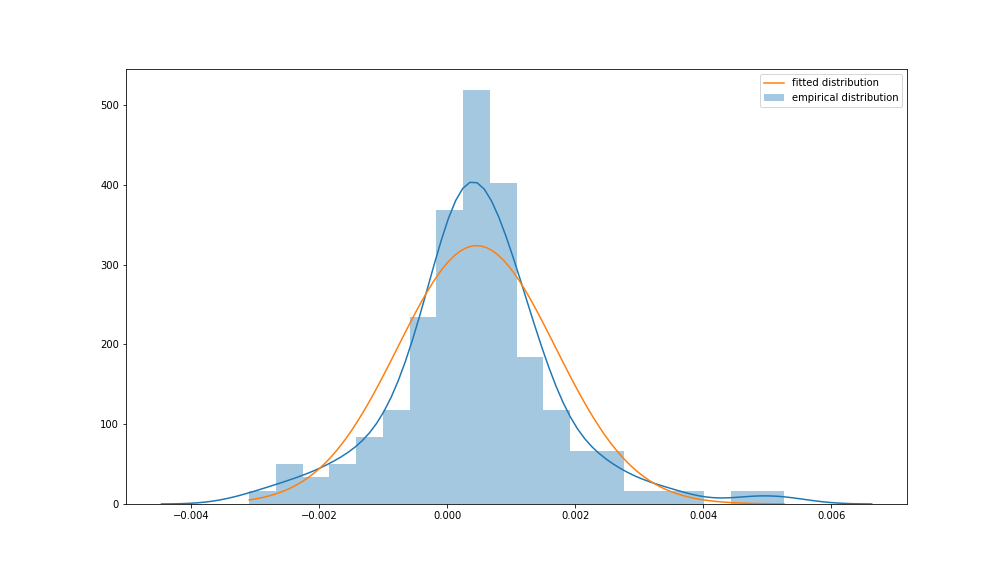
\includegraphics[scale=0.3]{figures/distribution_means.png}
\caption{Distribution of individual means $\mu_i^{(t)}$}
\label{fig:distmeans}
\end{figure}


\subsection{Sampling of covariance matrix}

Sampling the covariance matrix is more involved than sampling $\mu$. I go the following way about in in this paper: Realize that a transformation from a covariance matrix to a correlation matrix is possible:

\begin{equation}
    \text{corr}_{x, y} = \frac{\sigma_{x,y}^{2}}{\sigma_x \cdot \sigma_y}
\end{equation}

Therefore we first need to sample a correlation matrix, then a vector of variances, then transform the correlation matrix to the covariance matrix $\Omega^{(t)}$.

\subsubsection{Sampling of correlation matrix}

Sampling a correlation matrix is not as straightforward as sampling the individual stock returns, $\mu_i^{(t)}$. This is due to the fact, the correlation matrix should adhere to multiple criteria:

\begin{enumerate}
    \item A correlation matrix is a positive definite matrix.
    \item The individual values (apart from the diagonal) of the correlation matrix should follow a normal distribution $\rho_{i}^{(t)} \sim N(\kappa, \sigma_\rho)$.
\end{enumerate}

In this paper to accomplish the desired I use the following sampling scheme:

\begin{enumerate}
    \item Initialize an empty matrix $M$ of size $k \times k$.
    \item sample individual observations $\rho_{i,j}=\rho_{j,i}$ from a fitted normal distribtuion.
    \item Replace the diagonal of $M$ with 1.
    \item Save the matrix $M$ if all eigenvalues are positive, i.e. $M$ is positive definite.
\end{enumerate}

Figure \ref{fig:distcorrs} shows the fitted distribution plotted against the empirical distribution with regards to the individual $\rho_{i,j}^{(t)}$ not considering the diagonal. Again log-likelihood estimation is used to estimate the parameters: $\kappa=0.313, \sigma_\rho=0.188$. Again we see that, the actual distribution does not perfectly follow a normal distribution, but passes for a good approximation. It should be noted that when sampling from this distribution, the distribution is truncated at $(-1, 1)$.

\begin{figure}[ht]
\centering
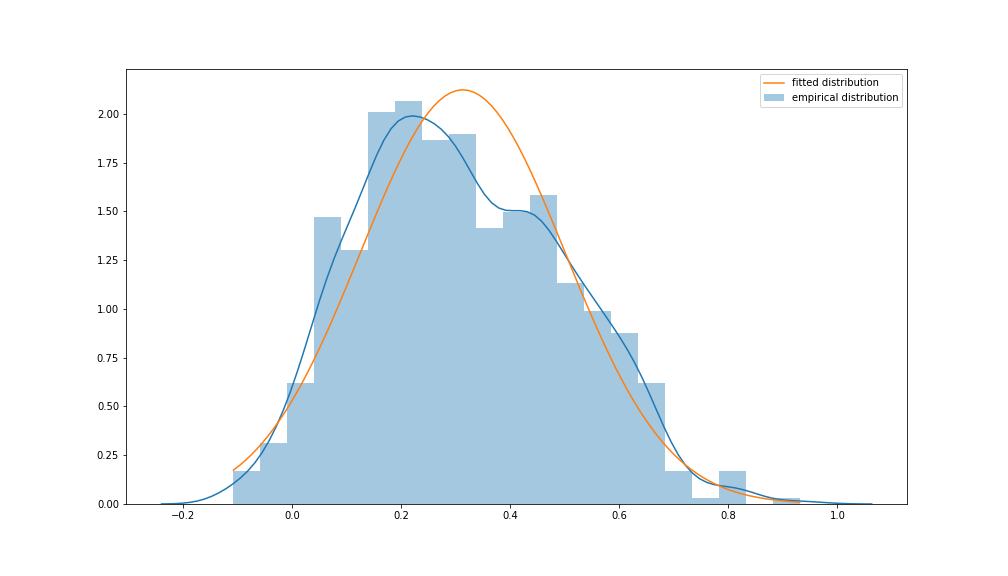
\includegraphics[scale=0.3]{figures/correlation_distribution.png}
\caption{Distribution of individual correlates $\rho_{i,j}^{(t)}$}
\label{fig:distcorrs}
\end{figure}

\subsubsection{Sampling of variances}

The variances does not follow a normal distribution, this is obvious, since the variance by definition is a positive measure. I model the variances to be exponentially distributed: $\sigma^2_{i} \sim expon(\lambda)$. Using log-likelihood estimation we find the $\lambda=0.000346$. Figure \ref{fig:distvars} displays the fitted distribution against the empirical distribution. I conclude that the exponential distribution is a reasonable approximation of the true distribution.

\begin{figure}[ht]
\centering
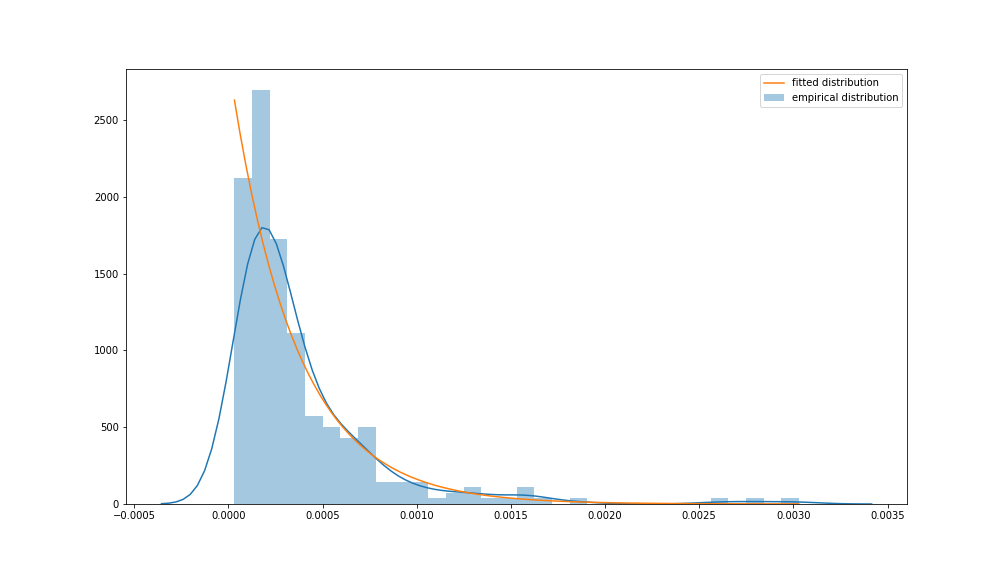
\includegraphics[scale=0.3]{figures/distribution_variances.png}
\caption{Distribution of individual variances}
\label{fig:distvars}
\end{figure}


\subsubsection{The simulated covariance distribution vs. the empirical distribution}

Using the scheme described above, I simulate a set of covariance matrices. Figure \ref{fig:distcovars} displays the simulated distribution of individual covariances vs. the empirical distribution of individual covariances. From the figure, we see that the simulated distribution, seems slightly biased towards 0. However I conclude that for the purpose of this paper the simulation passes as a good approximation.

\begin{figure}[ht]
\centering
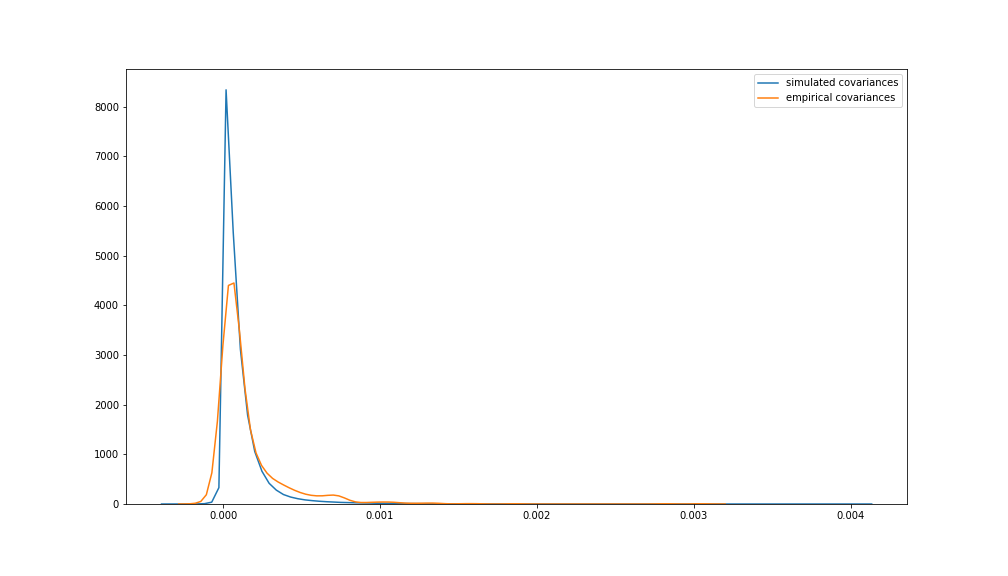
\includegraphics[scale=0.3]{figures/dist_simulated_covariances.png}
\caption{Distribution of individual covariances}
\label{fig:distcovars}
\end{figure}

\subsubsection{The simulated data set}

Now having simulated covariance matrices, and returns, we can simulate an entire data set, that corresponds to our model. We simulate a data set of $11$ columns and $2.000.0000$ rows, which is more than necessary for the further investigation in this paper. We set the parameter $p=0.047$, so we have just slightly less then $10.000$ structural breaks in the simulated data set. Since we have the underlying $\mu^{(t)}$ and $\Omega^{(t)}$ in each period, we can calculate the Sharpe ratios for each of the simulated stocks throughout the period assuming the risk free asset having a return of $\bar{r}=2 \%$ annually.

Summing it all up: A dataset is now constructed based on a structural model. The data set consists of not only the simulated returns, but also the Sharpe ratios of the individual stocks, which in the real data set are latent variables. The simulated data set allows for training, tuning and selecting between algorithms.



\section{Algorithms}

As mentioned earlier in this paper we investigate stock picking, by investing all assets in the single stock which yields highest Sharpe ratio at time $t$. Our ensemble of algorithms should therefore predict the Sharpe ratio for individual stocks.

For a given set of data: $\rr^{(t)} = (r_1^{(t)}, r_2^{(t)}, \cdots, r_k^{(t)})$, predict the sharp ratio: $f(\rr^{(t)}) = \mathbf{sr}^{(t)} = (sr_1^{(t)}, sr_2^{(t)}, \cdots, sr_k^{(t)}$), choose weights such that only $max$ of the Sharpe ratio is 1:
$\w^{(t)} = (0, 0, \cdots,0, 1, 0, \cdots, 0)$ which can be described by equation \ref{eq:maxsharp}.


\begin{equation}\label{eq:maxsharp}
    w_i^{(t)} =
    \begin{cases}
    1, &\text{if } \max({\mathbf{sr}^{(t)}}) = sr_i^{(t)} \\
    0, &\text{else}
    \end{cases}
\end{equation}.

\subsection{LSTM}

An LSTM (Long Short Term Memory) model is a deep neural network model that has proved itself extremely effective at explaining time series. Before delving into the inner workings of an LSTM it is useful to first present some general concepts of deep learning. Deep learning is a term used for deep neural networks. A neural network is an algorithm that has shown itself capable of representing extremely flexible functional forms. The network consists of layers: \textit{input layer, hidden layers, output layer}. Each layer consists of a number of units. The input layer takes some data input. The hidden layer makes a non linear transformation of these inputs. There can be multiple hidden layers, such that a hidden layer takes the output of a previous hidden layer as input. Lastly an output layer maps the hidden layers to some target. These deep neural networks usually contains many thousands (and in some cases millions) of parameters, these being biases and weights of the inputs to different units in the layers. These parameters are tuned by using a gradient descent algorithm. This can be done because the network is differentiable, and so it's possible to establish a loss function between the predicted target and the real target, that can be differentiated with respect to the parameters.

A special case of deep neural networks are recurrent neural networks. These networks are made for time series problems, where the input of the network in period $t$, is the output of the network in period $t-1$. LSTM models are subset of recurrent neural networks. LSTM models utilizes leaky units which is a way to represent longterm dependencies:

\begin{displayquote}

Leaky units allow the network to \textit{accumulate} information (such as evidence for a particular feature or category) over a long duration. Once that information has been used, however, it might be useful for the neural network to forget the old state. For example, if a sequence is made of subsequences and we want a leaky unit to accumulate evidence inside each sub-subsequence, we need a mechanism to forget the old state by setting it to zero. Instead of manually deciding when to clear the state, we want the neural network to learn to decide when to do it. This is what gated RNNs do \cite{goodfellow_deep_2016}.
\end{displayquote}

LSTM models contains cells of four different units: \textit{state unit, input gate, forget gate, output gate}. The \textit{state unit} represents the state of the network (or some part of the network) at period $t$. This cell has an internal recurrence. The \textit{forget gate} controls how this state evolves. This is done by controlling how much of the input should be transferred (or rather forgot) to the next state. The \textit{input gate} controls how much information should be accumulated into the current state. The \textit{output gate} controls how much of the state should be transferred forward. Figure \ref{fig:lstmcell} in the appendix show a representation of the cell.

\subsubsection{Architecture of network}

In this paper I have chosen a fairly standard LSTM architecture of a single LSTM layer with 256 outputs, and an output layer with 11 outputs, which represents the Sharpe ratios of the individual stocks. The input layer takes the returns for the individual stocks. The LSTM contains $277259$ trainable parameters. I train the network on sequences of length $250$. That is I sample sequences of $250$ consecutive observations from the simulated data, which the network can be trained on. I use \textit{mean squared error} (mse)\footnote{Equation \ref{eq:meansquarederror} shows how mean squared error is calculated} as the loss metric, where I let the network warm up for the first 50 observations in each sequence. Warming up implies not calculating the loss for the first 50 observations until the network has had time to represent the state of the system.

\subsection{Rolling Sharpe (Naive)}

The LSTM is a very complex algorithm, which even though they have proven themselves extremely effective at predicting difficult time series patterns, they have a tendency to be hard to train. To accommodate this challenge i propose this simpler algorithm.

Essentially this works by calculating the rolling Sharpe ratio for period of time for each stock, and using this as the prediction of the sharpe ratio. So for a given stock $s_i$ in period $t$ calculate the $\E[R_{i}^{(t)}]$ and $\std({R_{i}^{(t)}})$. And calculate the sharpe ratio by $(\E[R_{i}^{(t)}] - \bar{r}) / \std({R_{i}^{(t)}})$. Note that $\E[R_{i}^{(t)}] - \bar{r} = \E[R_{i}^{(t)} -\bar{r}^{(t)}]$ because $\bar{r}$ is constant throughout the period. The expectation and standard deviation is calculated as presented in equation \ref{eq:rs_mean_naive} and equation \ref{eq:rs_std_naive}.

\begin{equation}\label{eq:rs_mean_naive}
    \E[R_{i}^{(t)}] = \frac{1}{h}\sum_{i=0}^{h} r_{i}^{(t-i)}
\end{equation}

\begin{equation}\label{eq:rs_std_naive}
    \std (R_{i}^{(t)})  = \sqrt{\frac{1}{h}\sum_{i=0}^{h} \lp r_{i}^{(t-i)} - \E[R_{i}^{(t)}] \rp^{2}}
\end{equation}

where $h$ denotes the window length / the length of the memory of the algorithm. This hyper parameter $h$ can be tuned to get the best possible prediction of the Sharpe ratio.

This is called naive because this algorithm does not take structural breaks into account. Or in other words, this algorithm cannot forget its previous state even if it would be advantageous.

\subsection{Rolling Sharpe}

An extension to the naive approach is proposed to address the issue of the algorithm not being able to forget the previous state of the system, given a structural break happens.

Now consider we calculate the rolling Sharpe ratio as done above, but with the caveat it is now done for two different time periods, long term rolling Sharpe ratio and a short term rolling Sharpe ratio. In each period $t$ the algorithm stores to vectors of Sharpe ratios:

\begin{align}
    \mathbf{sr}^{(t)}_{\text{short term}} &= \lp \tilde{sr}_1^{(t)}, \tilde{sr}_2^{(t)}, \cdots , \tilde{sr}_k^{(t)}\rp \\
    \mathbf{sr}^{(t)}_{\text{long term}} &= \lp sr_1^{(t)}, sr_2^{(t)}, \cdots , sr_k^{(t)}\rp
\end{align}

where $\tilde{sr}$ is used to denote a sharpe ratio from the short term memory. A metrix can now be used to establish if the vectors $ \mathbf{sr}^{(t)}_{\text{short term}}$,  $ \mathbf{sr}^{(t)}_{\text{long term}}$ deviates to much. If it is the case they deviate to much, the long term memory is cleared and replaced  with the short term memory. The metric for this deviation of long and short term memory is calculated by equation \ref{eq:rs_distance}

\begin{equation}\label{eq:rs_distance}
    \text{Distance}_{sr^{(t)}} = \frac{1}{k}\sum_{i=1}^{k} \lp sr^{(t)}_{i} - \tilde{sr}^{(t)}_{i} \rp^{2}
\end{equation}

This algorithm has three hyper parameters: $h_{\text{long term}}$, $h_{\text{short term}}$, and lastly $\tau$, which is the threshold for the $\text{Distance}_{sr^{(t)}}$ where the long term memory of the algorithm is cleared.

The sharpe ratio is predicted using the long term memory the same way it was done for the naive version.


\section{Analysis}

\subsection{Algorithm selection}

To select algorithm I use the simulated dataset. This dataset contains the latent response variable (the Sharpe ratio of each stock). We evaluate algorithm by the lowest \textit{mean squared error (mse)} of Sharpe ratios.

\begin{equation}\label{eq:meansquarederror}
    mse = \sum_{t=1}^{T} \sum_{i=1}^{k}\lp \hat{sr}_{i}^{(t)} - sr_{i}^{(t)} \rp^2
\end{equation}

The algorithm with the lowest $mse$ is the algorithm selected to be tested on real data. Before testing each algorithm we need to tune, and in the case of the $LSTM$ train the algorithm. Training the algorithm consists of tuning the parameters that are endogenous to the algorithm, and tuning consists of finding the correct values for the hyper parameters.

The LSTM is trained by splitting the dataset into two separate parts (a training set and validation set). The LSTM is trained for 4 epochs, which is the number of times the LSTM goes through the entire training data.

The Naive Rolling Sharpe is tuned on 5000 observations, where a grid search over $h= \{50, 100, 150, 200, 250, 300\}$ is used. The $h$ which corresponds to lowest $mse$ is used for the final evaluation between the algorithms. We find that $h=200$ is the best hyper parameter value for the Naive Rolling Sharpe.

The Rolling Sharpe needs the three hyper parameters: $ h_{\text{long term}}$, $h_{\text{short term}}, \tau$. We create a grid of $3^3=27$ different values as shown in equation \ref{eq:rs_grid}. The algorithm is tuned over this grid, and we find the best hyper parameters to be $h_{\text{short term}} = 30, h_{\text{long term}} = 150, \tau = 30 $.

\begin{equation}\label{eq:rs_grid}
    grid = \underset{\tau}{\{0.3, 0.5, 0.8\}} \times \underset{h_{\text{long term}}}{\{50, 100, 150\}} \times \underset{h_{\text{short term}}}{\{15, 30, 45\}}
\end{equation}

Comparing the three trained and tuned algorithms on the same $5000$ observations yields: $MSE_{\text{LSTM}}= 0.0156$, $MSE_{\text{RS}_{naive}}= 0.0181$, $MSE_{\text{RS}}= 0.0131$. We conclude that the Rolling Sharpe algorithm performs the best. In the appendix figure \ref{fig:rollingsharptest} shows the underlying true Sharpe ratio for a given stock and the corresponding prediction made by the rolling Sharpe algorithm.


\subsection{Performance on real data}

Before applying the Rolling Sharpe algorithm on the real data, a couple of benchmark is established. The \textit{perfect stock pick} benchmark, is made by assuming that we as trader had perfect foresight over the next period, and was able to pick the stock in each period which yields the highest return. The second benchmark is the \textit{Apple} stock (with ticker \textbf{AAPL}). The Apple stock is chosen, since this is the stock with the highest individual Sharpe ratio of all the stocks throughout the period. The last benchmarks are two different tangency portfolios. One based on the first 1000 observations, and a tangency portfolio based on the entire period.

Equation \ref{eq:tangencyport} displays the formula for the tangency portfolio, where $\w$ is the weights of the portfolio, and: $\mu_{adj} = \mu - \bar{r}\cdot \mathbf{1}$. Which is the risk adjusted return. It should be noted that $\w$ is a vector of length $k$ and $\sum_{w \in \w} w = 1$.

\begin{equation}\label{eq:tangencyport}
    \w = \frac{\Omega^{-1} \cdot \mu_{adj}}{\mathbf{1}^{T} \cdot \Omega^{-1} \cdot \mu_{adj}}
\end{equation}

Looking to table \ref{tab:performance} we find that the rolling Sharpe algorithm performs very well. Comparing to \textbf{Apple} we find that the sharp ratio is 4 times higher, and the expected returns is over twice as high, and a somewhat lower standard deviation. Comparing to the tangency portfolio compared over the entire period we find the Sharpe ratio to be twice as high for the rolling Sharpe algorithm. The standard deviation of the tangency portfolio is lower than that of the rolling Sharpe algorithm. However that expected return from the rolling Sharpe algorithm is almost 4 times higher. Lastly comparing to tangency portfolio of only the first 1000 observations, which more realistically would represent how an investor would generate portfolio weights, i.e. the investor cannot use the future innovations of the data generating process to construct portfolio weights. Here again we find that the rolling Sharpe algorithm has 4 times as high Sharpe ratio.

\begin{table}[ht]
\centering
\caption{Summary statistics of performance of different portfolios}
\begin{tabular}{lrrr}
\toprule
{} &  Expected Return &      Std &  Sharpe Ratio \\
\midrule
rolling sharpe                &          0.00263 &  0.02028 &       0.12562 \\
perfect stock pick            &          0.02515 &  0.02285 &       1.09734 \\
apple                         &          0.00111 &  0.02824 &       0.03661 \\
tangency portfolio (1000 obs) &          0.00058 &  0.01830 &       0.02719 \\
tangency portfolio (all obs)  &          0.00077 &  0.01246 &       0.05545 \\
\bottomrule
\end{tabular}

\label{tab:performance}
\end{table}

Figure \ref{fig:loginvest} displays (the log transformed) portfolio given one had invested following the different benchmarks, using the real data. We see again that the rolling Sharpe ratio is by far the best way to invest throughout the period. Interestingly the poorest performing portfolio is the tangency portfolio calculated on the first 1000 observations.

\begin{figure}[ht]
\centering
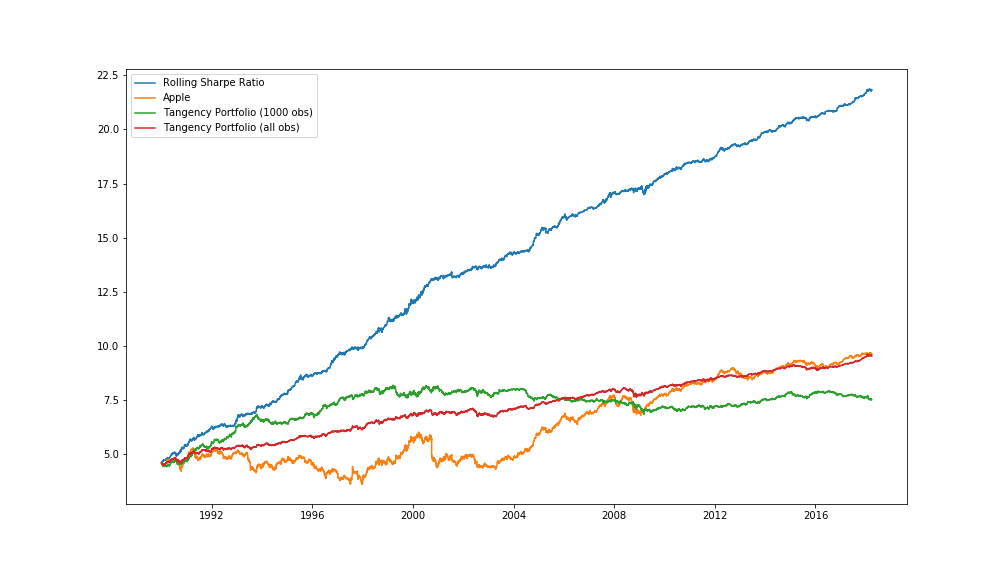
\includegraphics[scale=0.45]{figures/log_investment_experiment.png}
\caption{Counter factual portfolio performance (in logs)}
\label{fig:loginvest}
\end{figure}

Figure \ref{fig:logmontecarlo} uses Monte Carlo simulation to compare the different algorithms. By assuming that returns are normal distributed, we simulate portfolios following each of the four strategies: \textit{Rolling Sharpe, Apple Portfolio, Tangency portfolio (1000 obs), Tangency Portfolio (full)}. Since each portfolio have given both a mean and a standard deviation, we can use these distribution moments to randomly draw a return from given portfolio strategy. For each strategy we simulate 10000 portfolios. We run each portfolio for 7013 time steps.

\begin{figure}[ht]
\centering
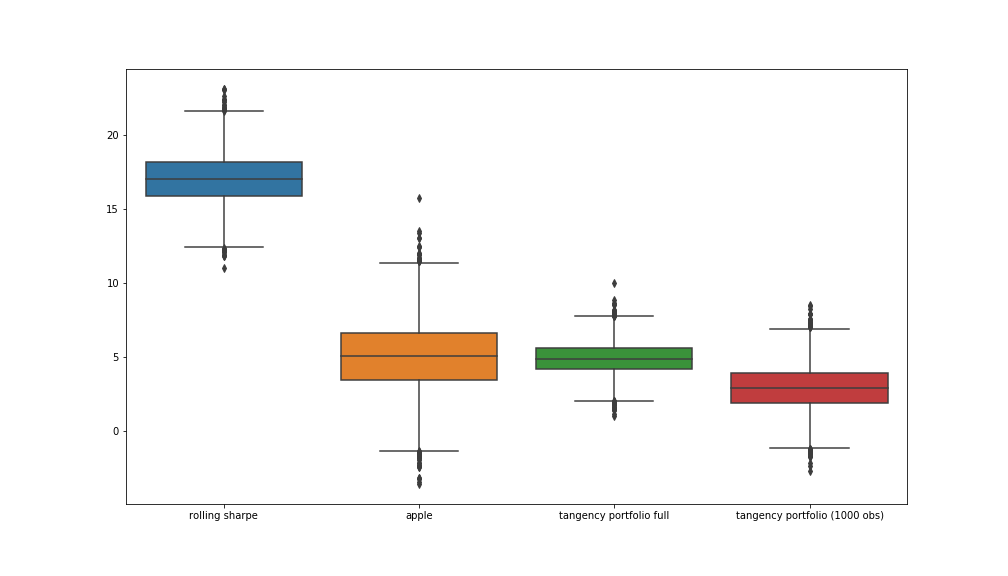
\includegraphics[scale=0.45]{figures/boxplot_monte_carlo.png}
\caption{Monte Carlo simulation - performance (in logs)}
\label{fig:logmontecarlo}
\end{figure}

Here we find again the rolling Sharpe algorithm performs best. The apple and tangency portfolio for the entire period seems to be doing approximately equal, comparing the mean, however, the variance is considerably lower for the tangency portfolio. Note the logarithmic \textit{y}-scale.


\section{Discussion}

\subsection{Structural Causal Models}

In this paper, we have assumed that the data generating process is governed by structural breaks. As alluded to in section \ref{sec:model}, another possibility would have been to assume a data generating process that followed something akin to an AR-process. Furthermore, other variables could have been assumed to influence the DGP of the simulated returns. When training, tuning and selecting between algorithms, I believe using multiple different ``environments'' is a good idea. Maybe one algorithm will perform well under certain circumstances and poorly under other. The use of controlled environments to develop and evaluate algorithms are highly beneficial, so testing the robustness under different assumptions would be an obvious extension to the work presented in this paper.

\subsection{LSTM challenges}

In this paper I tried implementing an LSTM. Getting this model to converge was a greater challenge than expected. This was due to multiple obstacles. First and foremost a LSTM is extremely slow to train on a CPU. I've used my personal computer to train the model. I could expect about 1 hour of training the model for each change to the architecture. If I had had access to a GPU (Graphical Processing Unit) the training could have been done considerably faster. These are however very expensive, and was infeasible for me to get hold on for this paper. GPU should be used in any further analysis using LSTM algorithms. LSTMs are very hard to train, and no matter what i did, it performed poorly. LSTMs are known for being hard to tune, but this was more difficult, than what I had expected.

\subsection{The (lack of) Feasibility of Machine Learning Models}

Having had a generated data set containing the latent variables, the true Sharpe ratio for individual stock  in each period, I have found that machine learning methods in general are hard to use. I've in the experimental phase of this paper, tried multiple algorithms and setups, and they have all had a hard time fitting the data in any usable way. This insight sheds light on the dangers of creating algorithms that perform well in-sample. Going forward building machine learning systems using only historical data, should be considered a risky business, and should be subject to a very thorough validation procedure, to be sure that the algorithm does not overfit the data.



\section{Conclusion}

This paper broadly follows three parts: First a structural causal model defining the data generating process of the returns of stocks was formulated. Using daily returns for 11 stock for the last 30 years, relevant statistics was calculated, and used for tuning the parameters of the DGP. Using the structural causal model a data set was simulated. 2) An ensemble of three algorithms that predicts the Sharpe ratio of individual stocks was presented. Using these three models, I tune, train and select an algorithm on the simulated data set. I find the best performing algorithm being a model that estimates the sharp ratio for individual stocks by storing a rolling set of observations and calculating the relevant moments using this memory. 3) Using the tuned algorithm we apply it out-of-sample to the real data. Using the rolling Sharpe algorithm I find (comparing it to 4) other benchmarks, the algorithm performs extremely well, having a Sharpe ratio at $0.1256$ comparing to a tangency portfolio with a Sharpe ratio of $0.05545$. I discuss the different challenges of tuning an LSTM, and the value of using a structural causal model as test environment for trading algorithms. Finally I point out the challenges of using machine learning models in-sample, and express a word of caution of doing so.


\section{Appendix}

\begin{figure}[ht]
\centering
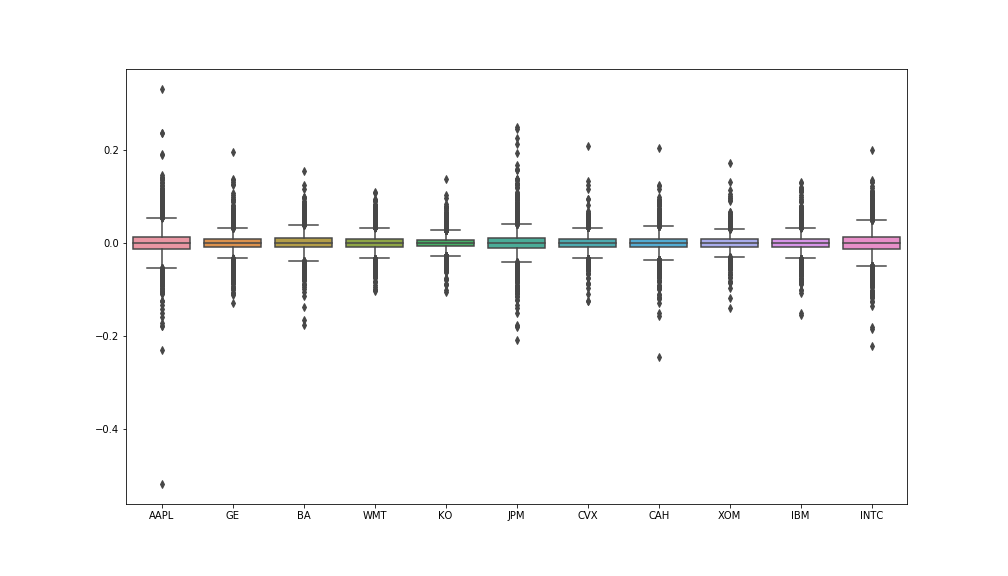
\includegraphics[scale=0.45]{figures/boxplot.png}
\caption{Boxplot of the daily returns for each stock}
\label{fig:returns_boxplots}
\end{figure}

\begin{figure}[ht]
\centering
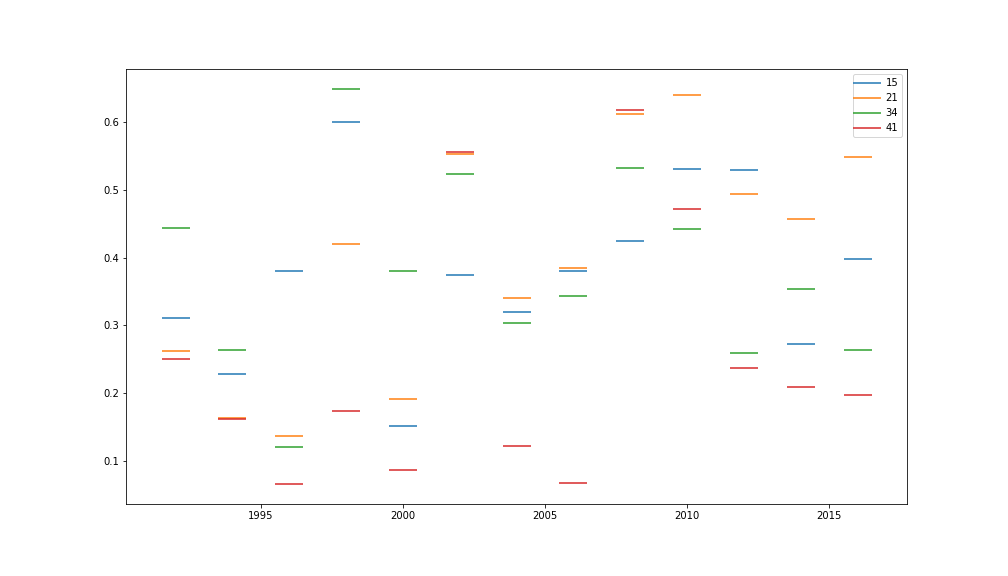
\includegraphics[scale=0.45]{figures/structural_breaks_covars.png}
\caption{Bi-annual covariances of 4 randomly chosen covariances}
\label{fig:structuralbreakscovariances}
\end{figure}

\begin{figure}[ht]
\centering
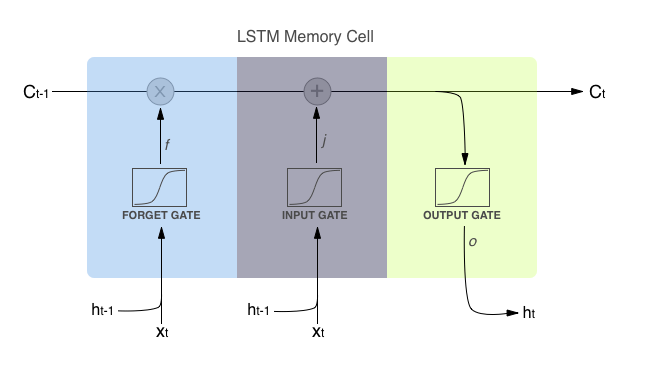
\includegraphics[scale=0.45]{figures/LSTM_cell.png}
\caption{LSTM cell}
\label{fig:lstmcell}
\end{figure}


\begin{figure}[ht]
\centering
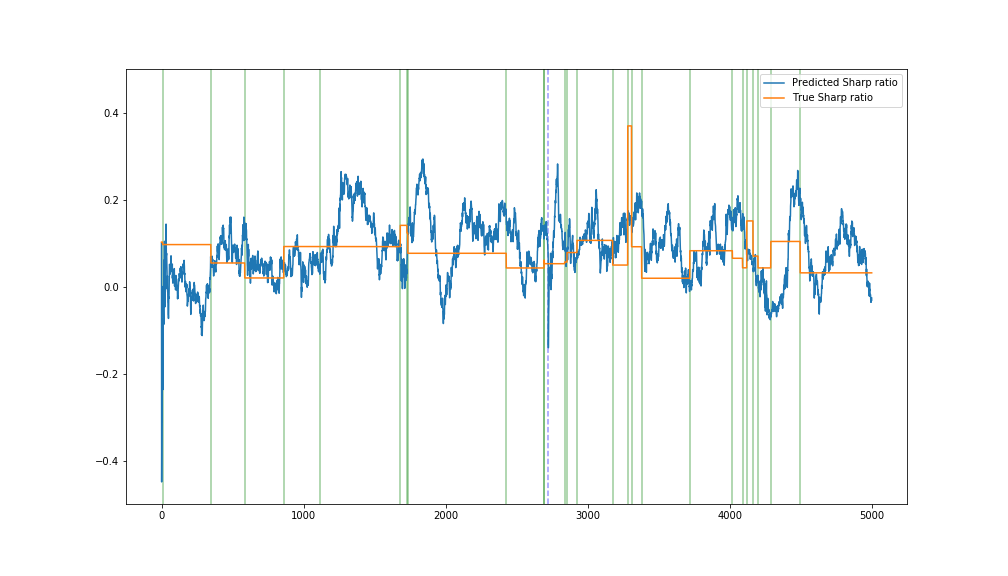
\includegraphics[scale=0.45]{figures/rolling_sharp_prediction_simulated.png}
\caption{LSTM cell}
\label{fig:rollingsharptest}
\end{figure}



\newpage
%\printbibliography

\end{document}
